\documentclass[12pt, a4paper]{article}
\usepackage{custom_config}
\numberwithin{equation}{subsection}

\begin{document}

{
	\LARGE Malkin Textbook Responses -- Final Report
}

{
	Gavin Kerr\\
	\today
}

\section{2-4 Malkin}
\textit{Explain why the value $\theta_K$, entering the Kohlrausch function, Eq. 2.1.6 is not a relaxation time. How do you find relaxation times for this relaxation function?}
\[
\varphi(t)=\exp\!\left[-\left(\frac{t}{\theta_K}\right)^n\right],
\qquad
\varphi(t)=\int_0^\infty G(\theta)\,e^{-t/\theta}\,d\theta.
\]
where $G(\theta)$ is the relaxation-time spectrum (what we want to find).
Let $s=1/\theta$, so $d\theta=-ds/s^2$,
\[
\varphi(t)=\int_0^\infty \frac{G(1/s)}{s^2}\,e^{-st}\,ds
\equiv \int_0^\infty \tilde G(s)\,e^{-st}\,ds,
\qquad
\tilde G(s)=\frac{G(1/s)}{s^2}.
\]
Therefore $\tilde G$ is obtained by an inverse Laplace transform:
\[
\tilde G(s)=\mathcal L^{-1}\{\varphi(t)\}(s)
=\frac{1}{2\pi i}\int_{\gamma-i\infty}^{\gamma+i\infty}
e^{st}\,\varphi(t)\,dt
\]
\[
\boxed{\tilde G(s)=
\frac{1}{2\pi i}\int_{\gamma-i\infty}^{\gamma+i\infty}
e^{st}\,e^{-(s_K t)^n}\,dt, \quad \text{where } s_K=1/\theta_K}
\]
But without solving, we can just say:
\[
\tilde G(s)=\mathcal L^{-1}\{\varphi(t)\}(s)
\implies
G(\theta)=\frac{\tilde G(1/\theta)}{\theta^2}.
\]
All together
\[
	G(\theta) = \frac{1}{\theta^2}\mathcal L^{-1}\left\{e^{-(s_K t)^n}\right\}(1/\theta).
\]

\subsection{Discrete relaxation times}
If we want a simple solution, we can assume a discrete set of relaxation times.
So we can write
\[
	G(\theta) = \sum_{i=1}^N G_i \delta(\theta - \theta_i)
\]
so that there are $T$ discrete relaxation times $\theta_i$ with weights $G_i$.
Then we have our relaxation function as:
\[
	\varphi(t) = \sum_{i=1}^N \int_0^\infty G_i \delta(\theta - \theta_i) e^{-t/\theta} d\theta
	= \sum_{i=1}^N G_i e^{-t/\theta_i}.
\]
Now we can equate this to the Kohlrausch function:
\[
	e^{- (t/\theta_K)^n }
	= \sum_{i=1}^N G_i e^{-t/\theta_i}.
\]


\subsection{Analytic solution}
Following Pollard (1946)\footnote{Pollard, H. (1946). The representation of $e^{-x^\lambda}$ as a Laplace integral.}, the inverse Laplace transform of 
\[
    \tilde{G}(s) = \frac{1}{2\pi i}
    \int_\gamma e^{st}\, e^{-(s_K t)^n}\, dt
\]
can be simplified to.
\begin{equation}
    \tilde{G}(s) =
    \frac{1}{\pi}\,\mathrm{Im}\left\{
    \sum_{k=1}^\infty \frac{(-1)^{k-1}}{k!}\,
    e^{-i\pi n k}\,
    \frac{\Gamma(nk+1)}{(s/s_K)^{nk+1}}
    \right\} \cdot \frac{1}{s_K}.
    \label{eq:pollard_series}
\end{equation}
The relaxation spectrum is therefore $G(\theta) = \tilde{G}(1/\theta)/\theta^2$:
\[
    G(\theta) = \frac{1}{\pi\,\theta}
    \,\mathrm{Im}\left\{
    \sum_{k=1}^\infty \frac{(-1)^{k-1}}{k!}\,
    e^{-i\pi n k}\,\Gamma(nk+1)
    \left(\frac{\theta}{\theta_K}\right)^{nk}
    \right\}.
\]

\begin{figure}[H]
	\centering
	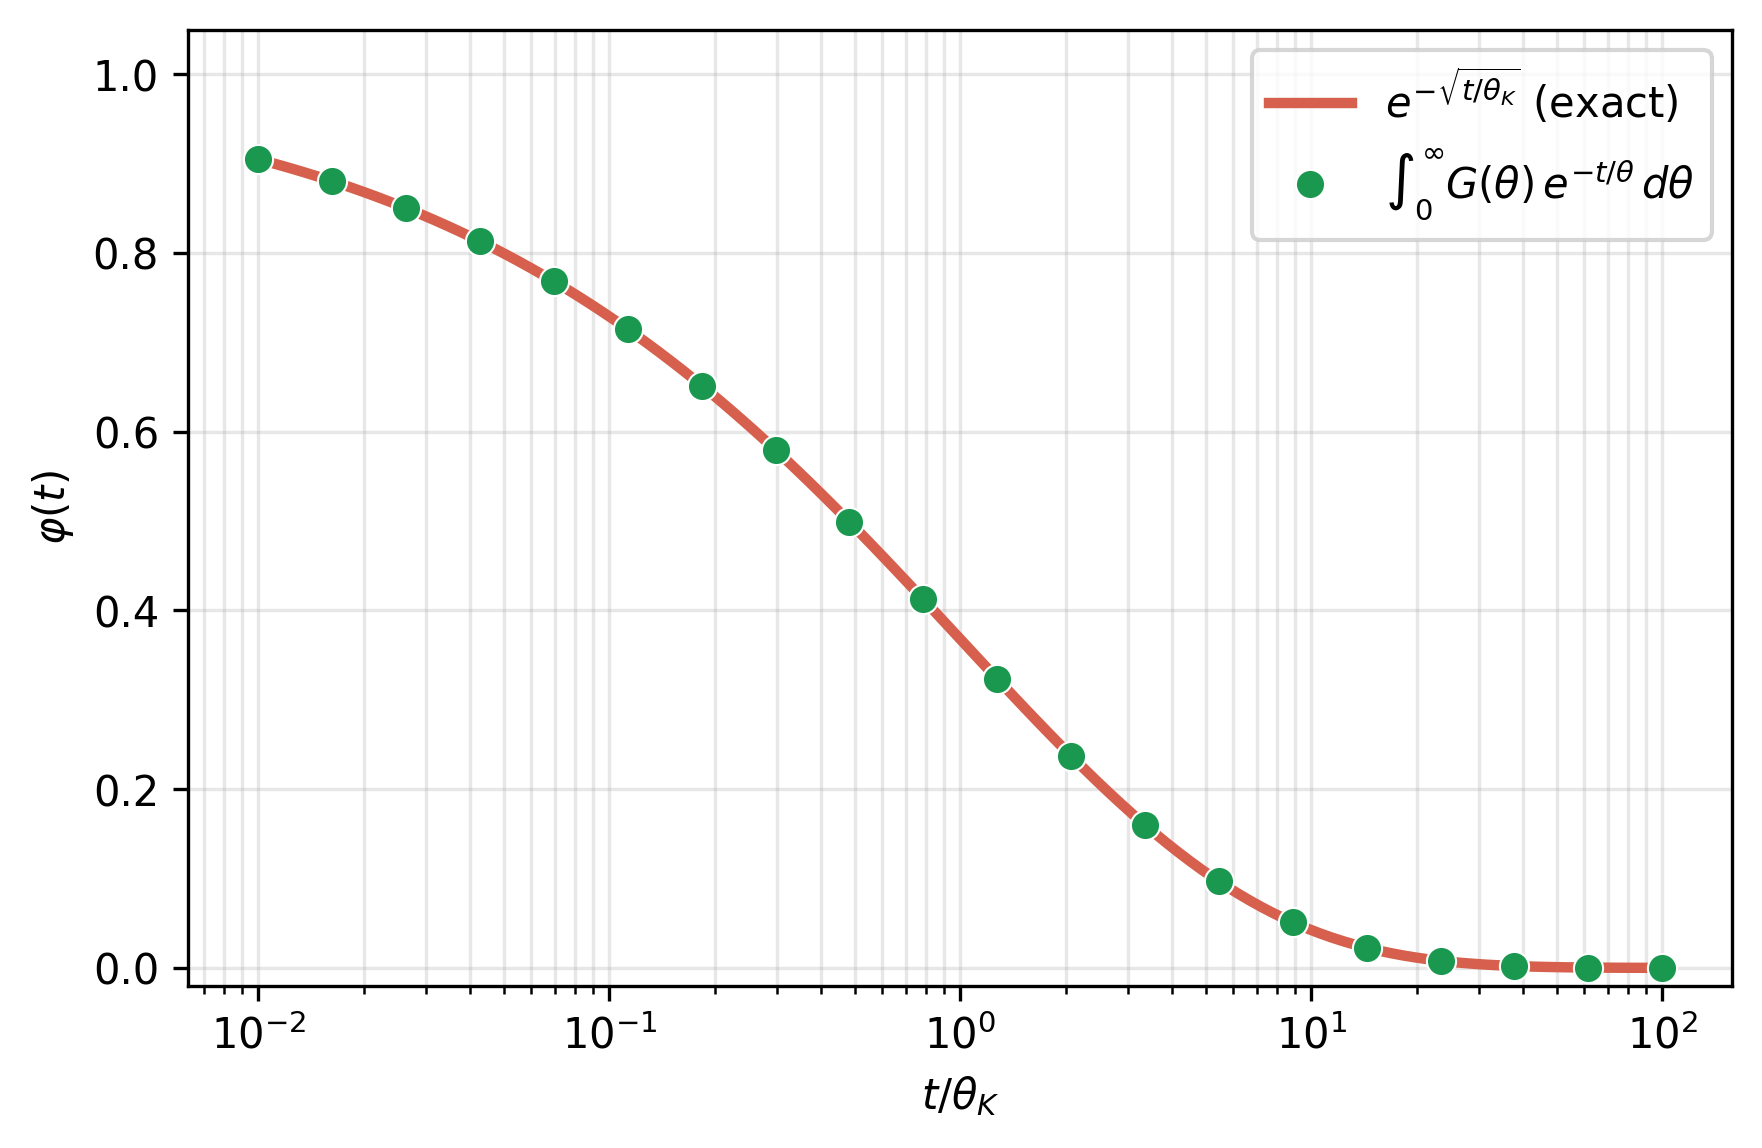
\includegraphics[width=0.7\textwidth]{figures/kww_half.png}
	\caption{
		Verification of the Pollard identity for $n=1/2$: $\varphi(t)=e^{-(t/\theta_K)^{1/2}}$.
	}
	\label{fig:kwww}
\end{figure}
In Figure~\ref{fig:kwww}, the relaxation function $\varphi(t) = e^{-\sqrt{t/\theta_K}}$ (solid line) the replicated by the numerical integration of equation~\ref{eq:pollard_series}.

%\subsection{Analytic Solution}
%We have
%\[
%\widetilde G(s)=\mathcal L^{-1}\left\{e^{-(s_K t)^n}\right\}(s),
%\qquad s_K=\frac{1}{\theta_K},\quad 0<n<1.
%\]
%Expand the stretched exponential:
%\[
%e^{-(s_K t)^n}=\sum_{k=0}^\infty \frac{(-1)^k}{k!}\,s_K^{nk}\,t^{nk}.
%\]
%Use the inverse Laplace transform identity
%\[
%\mathcal L^{-1}\{t^{a}\}(s)=\frac{1}{\Gamma(-a)}\,s^{-a-1}
%\]
%which can be obtained by analytic continuation of
%\(\mathcal L\{t^{\alpha-1}/\Gamma(\alpha)\}=s^{-\alpha}\).
%With \(a=nk\), this gives
%\[
%\mathcal L^{-1}\{t^{nk}\}(s)=\frac{1}{\Gamma(-nk)}\,s^{-nk-1}.
%\]
%Therefore
%\[
%\boxed{
%\widetilde G(s)
%=\sum_{k=0}^\infty \frac{(-1)^k}{k!}\,s_K^{nk}\,
%\frac{1}{\Gamma(-nk)}\,s^{-nk-1}.
%}
%\]
%
%\textbf{Convert back to the relaxation-time spectrum}
%
%Recall \(\widetilde G(s)=G(1/s)/s^2\), hence \(G(\theta)=\widetilde G(1/\theta)/\theta^2\).
%Substitute \(s=1/\theta\):
%\[
%\widetilde G(1/\theta)
%=\theta\sum_{k=0}^\infty \frac{(-1)^k}{k!}\,
%\frac{1}{\Gamma(-nk)}(s_K\theta)^{nk}.
%\]
%Thus
%\begin{equation}
%\boxed{
%G(\theta)
%=\frac{1}{\theta}\sum_{k=1}^\infty \frac{(-1)^k}{k!}\,
%\frac{1}{\Gamma(-nk)}\left(\frac{\theta}{\theta_K}\right)^{nk},
%\qquad (0<n<1).
%}
%\label{eq:relaxation_spectrum_kohlrausch}
%\end{equation}

%Does this converge?
%\[
%	\int_0^\infty G(\theta) d\theta
%	= \sum_{k=1}^\infty \frac{(-1)^k}{k! \Gamma(-nk)} \theta_K^{-nk} \int_0^\infty \theta^{nk - 1} d\theta
%\]
%We know that $0 < n < 1$, so $nk - 1 > -1$ for $k \geq 1$.
%Therefore the integral diverges:
%\[
%	= \sum_{k=1}^\infty \frac{(-1)^k}{k! \Gamma(-nk)} \theta_K^{-nk} \cdot \infty
%\]
% 
%\subsection{Simulation}
%When I try to simulate Eq. \ref{eq:relaxation_spectrum_kohlrausch} it doesn't converge well.
%This is likely because of the $\Gamma(-nk)$ term in the denominator which diverges for integer $nk$ and therefore isn't numerically stable.
%To fix this we use the Euler's reflection formula:
%\[
%	\Gamma(z) \Gamma(1 - z) = \frac{\pi}{\sin(\pi z)}
%	\implies
%	\Gamma(-nk) = \frac{-\pi}{\sin(\pi nk) \Gamma(1 + nk)}.
%\]
%Substituting this into Eq. \ref{eq:relaxation_spectrum_kohlrausch} gives:
%\[
%G(\theta)
%=\frac{1}{\theta}\sum_{k=1}^\infty \frac{(-1)^{k+1}}{k!}\,
%\frac{\sin(\pi nk)}{\pi}\,\Gamma(1+nk)
%\left(\frac{\theta}{\theta_K}\right)^{nk},
%\qquad (0<n<1).
%\]
%We can attempt to show numerically that
%\[
%	\int_0^\infty G(\theta) e^{-t/\theta} d\theta
%	\approx e^{-(t/\theta_K)^n}
%\]
%After trying this in python it \emph{does} blow up.


\section{2-8 Malkin}
\textit{Eq. 2.3.11 and its solution show that the \emph{Burgers model} describes the behavior of a material with two relaxation times. The same behavior is represented by two parallel Maxwell elements with their relaxation times $\theta_1 = n_1/G_1$ and $\theta_2 = n_2/G_2$ where $n_1$ and $G_1$ are the viscosity and elastic modulus of the first and $n_2$ and $G_2$ of the second Maxwell elements  joined in parallel. Calculate the values of the constants of the Burgers model expressed via constants of the two Maxwell elements.}

\subsection{Burgers Model:}
For the total strain rate we have:
\begin{equation*}
	\dot\gamma = \dot\gamma_m + \dot\gamma_k
	= \frac{\sigma}{\eta_m} + \frac{\dot\sigma}{G_m} + \dot\gamma_k.
\end{equation*}
\begin{equation*}
	\dot\gamma_k = \dot\gamma - \frac{\sigma}{\eta_m} - \frac{\dot\sigma}{G_m}, \quad
	\ddot\gamma_k = \ddot\gamma - \frac{\dot\sigma}{\eta_m} - \frac{\ddot\sigma}{G_m}.
	\label{eq:tot_strain_rate}
\end{equation*}
The stress across the Maxwell and Kelvin-Voigt elements is the same:
\begin{equation*}
	\sigma = \sigma_m = \sigma_k
	\implies
	\sigma = G_k\gamma_k + \eta_k \dot\gamma_k.
\end{equation*}
Now we can differentiate this then substitute Eq. \ref{eq:tot_strain_rate} into it:
\begin{equation*}
	\dot\sigma = G_k \dot\gamma_k + \eta_k \ddot\gamma_k.
\end{equation*}
\begin{equation*}
	\dot\sigma
	= G_k \left(\dot\gamma - \frac{\sigma}{\eta_m} - \frac{\dot\sigma}{G_m}\right)
	+ \eta_k \left(\ddot\gamma - \frac{\dot\sigma}{\eta_m} - \frac{\ddot\sigma}{G_m}\right).
\end{equation*}
Collecting terms gives:
\begin{equation}
	\frac{\eta_k}{G_m}\,\ddot\sigma
	+ \left(1 + \frac{G_k}{G_m} + \frac{\eta_k}{\eta_m}\right)\dot\sigma
	+ \frac{G_k}{\eta_m}\,\sigma
	= \eta_k\,\ddot\gamma + G_k\,\dot\gamma.
	\label{eq:burgers_model}
\end{equation}


\subsection{Two Maxwell Elements in Parallel:}
Consider branch 1, a Maxwell element with spring $G_1$ in series with dashpot $\eta_1$.
Within this Maxwell element the stress is the same in the spring and dashpot:
\[
	\sigma_1 = \sigma_{G_1} = \sigma_{\eta_1},
	\qquad
	\sigma_1 = G_1 \gamma_{G_1},
	\qquad
	\sigma_1 = \eta_1 \dot\gamma_{\eta_1}.
\]
Therefore,
\[
	\dot\gamma_{G_1} = \frac{\dot\sigma_1}{G_1},
	\qquad
	\dot\gamma_{\eta_1} = \frac{\sigma_1}{\eta_1}.
\]
Since the spring and dashpot are in series, strains add in branch 1:
\begin{align*}
	\dot\gamma_1 &= \dot\gamma_{G_1} + \dot\gamma_{\eta_1} \\
	&= \frac{\dot\sigma_1}{G_1} + \frac{\sigma_1}{\eta_1}.
\end{align*}
Let $D \equiv \frac{d}{dt}$\footnote{Thank you to Grecia for showing me this method.}, this may be written as
\begin{align*}
	\dot\gamma_1 &= \left(\frac{1}{G_1}D + \frac{1}{\eta_1}\right)\sigma_1
	= \frac{\eta_1 D + G_1}{G_1\eta_1}\,\sigma_1.
\end{align*}

Similarly for branch 2:
\begin{align*}
	\dot\gamma_2 &= \frac{\dot\sigma_2}{G_2} + \frac{\sigma_2}{\eta_2}
	= \left(\frac{1}{G_2}D + \frac{1}{\eta_2}\right)\sigma_2
	= \frac{\eta_2 D + G_2}{G_2\eta_2}\,\sigma_2.
\end{align*}
Since the two branches are in parallel, the total strain rate is the same in both branches:
\[
	\dot\gamma 
	= \frac{\eta_1 D + G_1}{G_1\eta_1}\,\sigma_1
	= \frac{\eta_2 D + G_2}{G_2\eta_2}\,\sigma_2.
\]
\[
	\sigma_1 = \frac{G_1\eta_1}{\eta_1 D + G_1}\,\dot\gamma,
	\qquad
	\sigma_2 = \frac{G_2\eta_2}{\eta_2 D + G_2}\,\dot\gamma.
\]
The total stress is the sum of the stresses in each branch:
\begin{align*}
	\sigma &= \sigma_1 + \sigma_2 \\
	\sigma &= \frac{G_1\eta_1}{\eta_1 D + G_1}\,\dot\gamma
	+ \frac{G_2\eta_2}{\eta_2 D + G_2}\,\dot\gamma \\
	\sigma &= \left(\frac{G_1\eta_1}{\eta_1 D + G_1}
	+ \frac{G_2\eta_2}{\eta_2 D + G_2} \right)\,\dot\gamma
	\\
	\sigma &= 
		\frac{G_1\eta_1(\eta_2 D + G_2)
	    + G_2\eta_2(\eta_1 D + G_1)} 
	    {(\eta_2 D + G_2)(\eta_1 D + G_1)} 
		\dot\gamma
	\\
	(\eta_2 D + G_2)(\eta_1 D + G_1) \sigma
		&= (G_1\eta_1(\eta_2 D + G_2)
	    + G_2\eta_2(\eta_1 D + G_1))
		\dot\gamma
	\\
	(\eta_1\eta_2 D^2
	+ (\eta_1 G_2 + \eta_2 G_1) D
	+ G_1 G_2)
	\ \sigma
		&= (G_1\eta_1\eta_2 D + G_1\eta_1G_2
	    + G_2\eta_2\eta_1 D + G_2\eta_2G_1)
		\dot\gamma
	\\
	\eta_1\eta_2 \ddot\sigma
	+ (\eta_1 G_2 + \eta_2 G_1) \dot\sigma
	+ G_1 G_2\sigma
		&= ((G_1\eta_1\eta_2 + G_2\eta_2\eta_1) D
	    + G_1\eta_1G_2 + G_2\eta_2G_1)
		\dot\gamma
\end{align*}
\begin{equation*}
	\eta_1\eta_2 \ddot\sigma
	+ (\eta_1 G_2 + \eta_2 G_1) \dot\sigma
	+ G_1 G_2\sigma
		= (G_1\eta_1\eta_2 + G_2\eta_2\eta_1) \ddot\gamma
	    + (G_1\eta_1G_2 + G_2\eta_2G_1)\dot\gamma	
\end{equation*}
Finally,
\begin{equation}
	\frac{\eta_1\eta_2}{G_1G_2} \ddot\sigma
	+ \frac{(\eta_1 G_2 + \eta_2 G_1)}{G_1G_2} \dot\sigma
	+ \sigma
		= \frac{\eta_1(G_1\eta_2 + G_2\eta_2)}{G_1G_2} \ddot\gamma
	    + (\eta_1 + \eta_2)\dot\gamma	
		\label{eq:two_maxwell_parallel_soln}
\end{equation}
using $\theta_i = \eta_i / G_i$:
\begin{equation}
	\theta_1 \theta_2 \ddot\sigma
	+ (\theta_1 + \theta_2) \dot\sigma
	+ \sigma
	= (\theta_1 + \theta_2) \ddot\gamma
	+ (\theta_1 G_1 + \theta_2 G_2)\dot\gamma
\end{equation}
gives us a cleaner form.

\subsection{Equating Coefficients}
From Eq. \ref{eq:two_maxwell_parallel_soln} we have
\[
	\frac{\eta_1\eta_2}{G_1G_2} \ddot\sigma
	+ \frac{(\eta_1 G_2 + \eta_2 G_1)}{G_1G_2} \dot\sigma
	+ \sigma
		= \frac{\eta_1\eta_2(G_1 + G_2)}{G_1G_2} \ddot\gamma
			    + (\eta_1 + \eta_2)\dot\gamma
\]
From Eq. \ref{eq:burgers_model} we have
\[
	\frac{\eta_k}{G_m}\,\ddot\sigma
	+ \left(1 + \frac{G_k}{G_m} + \frac{\eta_k}{\eta_m}\right)\dot\sigma
	+ \frac{G_k}{\eta_m}\,\sigma
	= \eta_k\,\ddot\gamma + G_k\,\dot\gamma.
\]
So we can compare the two equations, we'll multiply Eq. \ref{eq:burgers_model} by $\frac{\eta_m}{G_k}$:
\[
	\frac{\eta_k \eta_m}{G_m G_k}\,\ddot\sigma
	+ \left(\frac{\eta_m}{G_k} + \frac{\eta_m}{G_m} + \frac{\eta_k}{G_k}\right)\dot\sigma
	+ \sigma
	= \frac{\eta_k \eta_m}{G_k}\,\ddot\gamma + \eta_m\,\dot\gamma.
\]
From left to right, we equate coefficients:
\begin{align}
	\frac{\eta_1\eta_2}{G_1G_2}
	&= \frac{\eta_k \eta_m}{G_m G_k} \label{eq:coeff1} \\
	\frac{(\eta_1 G_2 + \eta_2 G_1)}{G_1G_2}
	&= \frac{\eta_m}{G_k} + \frac{\eta_m}{G_m} + \frac{\eta_k}{G_k} \label{eq:coeff2} \\
	\frac{\eta_1\eta_2(G_1 + G_2)}{G_1G_2}
	&= \frac{\eta_k \eta_m}{G_k} \label{eq:coeff3} \\
	(\eta_1 + \eta_2)
	&= \eta_m \label{eq:coeff4}
\end{align}
Firstly we have the trivial result from Eq. \ref{eq:coeff4}:
\begin{equation*}
	\boxed{\eta_m = \eta_1 + \eta_2}.
\end{equation*}
Theoretically, we also have
\begin{equation*}
	G_m = G_1 + G_2
\end{equation*}
but we can show this by plugging Eq. \ref{eq:coeff1} into Eq. \ref{eq:coeff3}:
\begin{align*}
	\frac{\eta_1\eta_2}{G_1G_2}(G_1 + G_2)
	&= \frac{\eta_k \eta_m}{G_k} \\
	\frac{\eta_k \eta_m}{G_m G_k}(G_1 + G_2)
	&= \frac{\eta_k \eta_m}{G_k} \\
\end{align*}
\begin{equation*}
	\boxed{G_m = G_1 + G_2}.
\end{equation*}

Using $\eta_m=\eta_1+\eta_2$, $G_m=G_1+G_2$, and
\[
	\frac{\eta_k}{G_k}
	=
	\frac{\eta_1\eta_2(G_1+G_2)}{G_1G_2(\eta_1+\eta_2)},
\]

we can substitute into Eq. \ref{eq:coeff2} to solve for $G_k$:
\begin{align*}
	\frac{\eta_m}{G_k}
	&=
	\frac{\eta_1 G_2 + \eta_2 G_1}{G_1G_2}
	-\frac{\eta_1+\eta_2}{G_1+G_2}
	-\frac{\eta_1\eta_2(G_1+G_2)}{G_1G_2(\eta_1+\eta_2)}.
	\\
	\frac{\eta_m}{G_k}
	&=
	\frac{
	(\eta_1G_2+\eta_2G_1)(G_1+G_2)(\eta_1+\eta_2)
	- G_1G_2(\eta_1+\eta_2)^2
	- \eta_1\eta_2(G_1+G_2)^2
	}{
	G_1G_2(G_1+G_2)(\eta_1+\eta_2)
	}.
\end{align*}
Now expand the first term in the numerator:
\begin{align*}
	(\eta_1G_2+\eta_2G_1)(\eta_1+\eta_2)
	&=
	\eta_1^2G_2 + \eta_1\eta_2G_2 + \eta_1\eta_2G_1 + \eta_2^2G_1 \\
	&=
	\eta_1^2G_2 + \eta_2^2G_1 + \eta_1\eta_2(G_1+G_2).
\end{align*}
So
\begin{align*}
	(\eta_1G_2+\eta_2G_1)(G_1+G_2)(\eta_1+\eta_2)
	&=
	(G_1+G_2)\bigl[\eta_1^2G_2 + \eta_2^2G_1 + \eta_1\eta_2(G_1+G_2)\bigr] \\
	&=
	(G_1+G_2)(\eta_1^2G_2 + \eta_2^2G_1) + \eta_1\eta_2(G_1+G_2)^2.
\end{align*}
Substitute this back into the numerator; the $\eta_1\eta_2(G_1+G_2)^2$ terms cancel:
\begin{align*}
	\text{numerator}
	&=
	\Bigl[(G_1+G_2)(\eta_1^2G_2 + \eta_2^2G_1) + \eta_1\eta_2(G_1+G_2)^2\Bigr]\\
	&- G_1G_2(\eta_1+\eta_2)^2
	- \eta_1\eta_2(G_1+G_2)^2 \\
	&=
	(G_1+G_2)(\eta_1^2G_2 + \eta_2^2G_1) - G_1G_2(\eta_1+\eta_2)^2.
\end{align*}
Expand the remaining pieces:
\begin{align*}
	(G_1+G_2)(\eta_1^2G_2 + \eta_2^2G_1)
	&=
	\eta_1^2G_1G_2 + \eta_1^2G_2^2 + \eta_2^2G_1^2 + \eta_2^2G_1G_2, \\
	G_1G_2(\eta_1+\eta_2)^2
	&=
	G_1G_2(\eta_1^2 + 2\eta_1\eta_2 + \eta_2^2)
	=
	\eta_1^2G_1G_2 + 2\eta_1\eta_2G_1G_2 + \eta_2^2G_1G_2.
\end{align*}
Subtracting gives
\begin{align*}
	\text{numerator}
	&=
	(\eta_1^2G_2^2 + \eta_2^2G_1^2) - 2\eta_1\eta_2G_1G_2
	=
	(G_1\eta_2 - G_2\eta_1)^2.
\end{align*}
then
\begin{equation*}
	\frac{\eta_m}{G_k}
	=
	\frac{(G_1\eta_2 - G_2\eta_1)^2}{G_1G_2(G_1+G_2)(\eta_1+\eta_2)}.
\end{equation*}
Since $\eta_m=\eta_1+\eta_2$, invert to obtain
\begin{equation*}
	\boxed{
	G_k=
	\frac{G_1G_2\,(G_1+G_2)\,(\eta_1+\eta_2)^2}{(G_1\eta_2-G_2\eta_1)^2}
	}.
\end{equation*}
Finally, using Eq. \ref{eq:coeff1} $\eta_k/G_k=\eta_1\eta_2(G_1+G_2)/[G_1G_2(\eta_1+\eta_2)]$, we can solve for $\eta_k$:
\begin{equation*}
	\eta_k
	=
	G_k\frac{\eta_k}{G_k}
	=
	\left[\frac{G_1G_2\,(G_1+G_2)\,(\eta_1+\eta_2)^2}{(G_1\eta_2-G_2\eta_1)^2}\right]
	\left[\frac{\eta_1\eta_2(G_1+G_2)}{G_1G_2(\eta_1+\eta_2)}\right],
\end{equation*}
so
\begin{equation*}
	\boxed{
	\eta_k=
	\frac{\eta_1\eta_2\,(G_1+G_2)^2\,(\eta_1+\eta_2)}{(G_1\eta_2-G_2\eta_1)^2}
	}.
\end{equation*}

\section{3-5 and 3-6 Malkin}
\textit{3-5: Calculate shear stresses in the flow of liquid through a straight tube if the flow is created by the pressure gradient $\Delta p/L$ ($L$ is the length of a tube).}

\textit{3-6: Calculate the radial distribution of shear rates and flow velocity of Newtonian liquid (having viscosity $\eta$) through a straight tube with radius $R$.}

I decided to combine these because the first first part of 3-6 entirely answers 3-5.

Starting with the \emph{Navier-Stokes equation}:
\[
	\rho \left( \frac{\partial \mathbf{u}}{\partial t} + (\mathbf{u}\cdot\nabla)\mathbf{u} \right) = -\nabla p + \nabla\cdot\boldsymbol{\sigma}.
\]
Evaluating the left-hand side, we have the following due to the steady flow assumption:
\[
	\frac{\partial \mathbf{u}}{\partial t} = 0.
\]
And for the other LHS term:
\[
	((\mathbf{u}\cdot\nabla)\mathbf{u})_i
	= u_j \partial_j u_i
	= u_r \partial_r u_i + u_\theta \tfrac1r\partial_\theta u_i + u_z \partial_z u_i
\]
$u_r = u_\theta = 0$ therefore
\[
	((\mathbf{u}\cdot\nabla)\mathbf{u})_r = 
	((\mathbf{u}\cdot\nabla)\mathbf{u})_\theta = 0
\]
$\mathbf{u} = u_z(r)$
\[
	((\mathbf{u}\cdot\nabla)\mathbf{u})_i
	= u_r \partial_r u_z + u_\theta \tfrac1r\partial_\theta u_z + u_z \partial_z u_z = 0
\]
Therefore the whole LHS of the Navier Stokes is zero. Navier-Stokes equation reduces to
\[
	\nabla p = \nabla\cdot\boldsymbol{\sigma}.
\]
In cylindrical coordinates, the RHS is 
\[
	\nabla\cdot\boldsymbol{\sigma} = 
	\frac{1}{r}\frac{\partial}{\partial r}(r\sigma_{rz}) + 
	\frac{1}{r}\frac{\partial \sigma_{\theta z}}{\partial \theta} + 
	\frac{\partial \sigma_{zz}}{\partial z}
	= \frac{1}{r}\frac{\partial}{\partial r}(r\sigma_{rz}).
\]
All other terms are zero since $\sigma_{\theta z} = 0$ and $\sigma_{zz}$ is independent of $z$ for steady flow. The pressure gradient is constant, so $\nabla p = \frac{\Delta P}{L}$, and we have
\begin{align*}
	\frac{\Delta P}{L} &= \frac{1}{r}\frac{\partial}{\partial r}(r\sigma_{rz})\\
	\frac{\Delta P}{L}\, r &= \frac{\partial}{\partial r}(r\sigma_{rz})\\
	\int \frac{\Delta P}{L}\, r\,dr
	&= \int \frac{\partial}{\partial r}(r\sigma_{rz})\,dr\\
	\frac{\Delta P}{L}\frac{r^2}{2} + C_1
	&= r\sigma_{rz}.
\end{align*}

Solving for the shear stress gives
\[
	\sigma_{rz}
	=
	\frac{\Delta P}{2L} r + \frac{C_1}{r}.
\]

The stress must remain finite at the centerline $r=0$, which requires $C_1 = 0$. Therefore
\[
	\boxed{\sigma_{rz} = \frac{\Delta P}{2L}\, r}.
\]

This is a key result: the shear stress $\sigma_{rz}$ is proportional to the radius $r$ and does not depend on the viscosity $\eta$.

Now we can use the constitutive relation for a Newtonian fluid $\sigma_{rz} = \eta \dot\gamma_{rz}$ to find the shear rate distribution:
\[
	\dot\gamma_{rz}
	=
	\frac{\sigma_{rz}}{\eta}
	=
	\frac{\Delta P}{2\eta L} r.
\]

Integrating the shear rate gives the velocity distribution:
\begin{align*}
	u_z(r)
	&=
	\int \dot\gamma_{rz}\,dr \\
	&=
	\int \frac{\Delta P}{2\eta L} r\,dr \\
	&=
	\frac{\Delta P}{4\eta L} r^2 + C_2.
\end{align*}

Applying the no-slip boundary condition $u_z(R) = 0$ gives
$C_2 = -\frac{\Delta P}{4\eta L} R^2,$
so the velocity profile becomes
\[
	\boxed{
	u_z(r) =
	\frac{\Delta P}{4\eta L}\,(r^2 - R^2)
	}.
\]

\textbf{Additional question 1.} \textit{Calculate the volume output, $Q$, for the flow of Newtonian liquid.}

The flow rate is given by
\[
	Q = \int \mathbf{u} \cdot d\mathbf{S}.
\]
All of the flow field $\mathbf{u}$ has the same direction as the outlet $S$ so
\[
	Q = \int u\, dS.
\]
The surface is just the cross sectional area of the pipe:
\[
	Q = \int_0^R \int_0^{2\pi} u\, r\, dr\, d\theta
	  = 2\pi\int_0^R  u\, r\, dr
\]
\[
	Q = 2\pi  \frac{\Delta P}{4\eta L}\int_0^R\,(r^2 - R^2) r dr
\]
\[
	\int_0^R r^3 dr = \frac{R^4}{4}, \quad
	R^2 \int_0^R r dr = \frac{R^4}{2}
\]
\[
	Q = 2\pi  \frac{\Delta P}{4\eta L}
	\left(\frac{R^4}{4} - \frac{R^4}{2}\right)
	= \boxed{\frac{\pi \Delta P R^4}{8\eta L}}
\]

\textbf{Additional question 2.} \textit{Express maximum shear rate via volume output.}
From earlier we have:
\[
	\sigma_{rx} = \frac{\Delta P r}{2 L}.
\]
$r\in[0,R]$, therefore:
\[
	\sigma_\text{max} = \frac{\Delta P R}{2 L}.
\]
\[
	Q = \frac{\pi R^3}{4\eta} \frac{\Delta P R}{2 L} = \frac{\pi R^3}{4\eta} \sigma_\text{max}
	\implies \sigma_\text{max} =  \boxed{\frac{4\eta Q}{\pi R^3}}
\]


\textbf{Additional question 3.} \textit{Is the last expression valid for a liquid with arbitrary rheological properties?}

No, in our derivation we assumed that $\sigma \propto \dot\gamma$. If we violate that assumption, we would need to modify our equation accordingly.

\section{3-9 Malkin}
\textit{Analyze the flow of a viscoplastic (``Bingham-type'') liquid through a straight tube of radius $R$. Find radial stress and velocity distributions and calculate volume output as a function of the pressure gradient.}

According to Malkin, the \textit{Bingham Equation} is
\begin{equation}
	\sigma = \sigma_Y + \mu \dot\gamma,
	\label{eq:bingham}
\end{equation}
where $\sigma_Y$ is the yield stress and $\mu$ is the plastic viscosity.
Or equivalently,
\[
	\dot\gamma = \begin{cases}
		0 & \text{if } \sigma < \sigma_Y \\
		\frac{\sigma - \sigma_Y}{\mu} & \text{if } \sigma \geq \sigma_Y
	\end{cases}.
\]

The stress distribution follows the same argument as in 3-5/3-6, giving
\[
    \sigma_{rz} = \frac{\Delta P}{2L}\, r.
\]

Flow only occurs when $\sigma(r) \geq \sigma_Y$, so there is a region in the center of the tube where $r < r_0$ for which there is no shearing.
The radius $r_0$ is given by:
\[
	\sigma(r_0) = \sigma_Y \implies r_0 = \frac{2L}{\Delta P}\sigma_Y.
\]

Recalling that for our ``Bingham fluid'' $\sigma = \sigma_Y + \mu \dot\gamma$, we can write $\dot\gamma$ as
\[
	\dot\gamma = \frac{\sigma - \sigma_Y}{\mu}
	= \frac{\Delta P}{2\mu L}r - \frac{\sigma_Y}{\mu}.
\]

Adding the requirement that $\dot\gamma = 0$ for $r < r_0$ gives the full shear rate distribution:
\[
	\boxed{\dot\gamma = \begin{cases}
		0 & r < r_0 \\
		\frac{\Delta P}{2\mu L}r - \frac{\sigma_Y}{\mu} & r \geq r_0
	\end{cases}}.
\]

As you increase $r$, the velocity $u_z$ decreases, so the shear rate $\dot\gamma$ is negative. Therefore,
\[
	\dot\gamma  = - \frac{du_z}{dr} \implies du_z = -\dot\gamma dr.
\]

Now we can integrate to get the velocity distribution in the region $r \geq r_0$:
\[
	u_z = -\int \dot\gamma dr
		= -\int \left(\frac{\Delta P}{2\mu L}r - \frac{\sigma_Y}{\mu}\right) dr
		= -\frac{\Delta P}{4\mu L}r^2 + \frac{\sigma_Y}{\mu}r + C.
\]

From the zero slip condition at the wall, we have
\[
	0 = -\frac{\Delta P}{4\mu L}R^2 + \frac{\sigma_Y}{\mu}R + C
	\implies C = - \frac{\sigma_Y}{\mu}R + \frac{\Delta P}{4\mu L}R^2.
\]

Therefore, the velocity distribution in the region $r \geq r_0$ is
\[
	u_z(r) = \frac{\Delta P}{4\mu L}(R^2 - r^2) - \frac{\sigma_Y}{\mu}(R - r).
\]

For the region $r < r_0$, there is no shearing, so the velocity is constant. The value of this constant is given by the velocity at $r = r_0$:
\[
	u_z(r) = \frac{\Delta P}{4\mu L}(R^2 - r_0^2) - \frac{\sigma_Y}{\mu}(R - r_0).
\]

Recall that
\[
	r_0 = \frac{2L}{\Delta P}\sigma_Y \implies \sigma_Y = \frac{\Delta P}{2L}r_0,
\]
so
\[
	\frac{\sigma_Y}{\mu}(R - r_0)
	=
	\frac{\Delta P}{2\mu L}r_0(R - r_0).
\]

Substituting this into the velocity expression gives
\[
	u_z(r)
	=
	\frac{\Delta P}{4\mu L}(R^2 - r_0^2)
	-
	\frac{\Delta P}{2\mu L}r_0(R - r_0)
	=
	\frac{\Delta P}{4\mu L}
	\left[
	(R^2 - r_0^2) - 2r_0(R - r_0)
	\right].
\]
\[
	=
	\frac{\Delta P}{4\mu L}
	(R^2 - 2Rr_0 + r_0^2)
	=
	\frac{\Delta P}{4\mu L}
	(R - r_0)^2.
\]

Then the full velocity distribution is
\[
	\boxed{u_z(r) = \begin{cases}
		\frac{\Delta P}{4\mu L}(R - r_0)^2 & r < r_0 \\
		\frac{\Delta P}{4\mu L}(R^2 - r^2) - \frac{\sigma_Y}{\mu}(R - r) & r \geq r_0
	\end{cases}}.
\]

Finally, we can calculate the volume flow $Q$ by integrating the velocity profile across the cross-sectional area of the tube. Since $d\mathbf{A} = r\,dr\,d\theta\,\hat{z}$ and $\mathbf{u} = u_z(r)\hat{z}$, we have
\begin{align*}
Q
&= 2\pi \int_0^R u_z(r)\, r\,dr \\
&= 2\pi \left[
\int_0^{r_0} \frac{\Delta P}{4\mu L}(R - r_0)^2 r\,dr
+ \int_{r_0}^R \left(\frac{\Delta P}{4\mu L}(R^2 - r^2) - \frac{\sigma_Y}{\mu}(R - r)\right) r\,dr
\right].
\end{align*}

For the region $(0 \le r \le r_0)$:
\begin{align*}
\int_0^{r_0} \frac{\Delta P}{4\mu L}(R - r_0)^2 r\,dr
&= \frac{\Delta P}{4\mu L}(R - r_0)^2 \int_0^{r_0} r\,dr \\
&= \frac{\Delta P}{4\mu L}(R - r_0)^2 \left[\frac{r^2}{2}\right]_0^{r_0} \\
&= \frac{\Delta P}{8\mu L}(R - r_0)^2 r_0^2.
\end{align*}

For the region $(r_0 \le r \le R)$:
\begin{align*}
\int_{r_0}^R \left(\frac{\Delta P}{4\mu L}(R^2 - r^2) - \frac{\sigma_Y}{\mu}(R - r)\right) r\,dr
&= \int_{r_0}^R
\left[
\frac{\Delta P}{4\mu L}(R^2 r - r^3)
- \frac{\sigma_Y}{\mu}(Rr - r^2)
\right]dr.
\end{align*}

Integrate term-by-term:
\begin{align*}
\int R^2 r\,dr &= R^2\frac{r^2}{2}, \qquad
\int r^3\,dr = \frac{r^4}{4}, \\
\int Rr\,dr &= R\frac{r^2}{2}, \qquad
\int r^2\,dr = \frac{r^3}{3}.
\end{align*}

Plugging the integrals back in gives
\begin{align*}
&\int_{r_0}^R \left(\frac{\Delta P}{4\mu L}(R^2 - r^2) - \frac{\sigma_Y}{\mu}(R - r)\right) r\,dr \\
&=
\left[
\frac{\Delta P}{4\mu L}\left(R^2\frac{r^2}{2} - \frac{r^4}{4}\right)
- \frac{\sigma_Y}{\mu}\left(R\frac{r^2}{2} - \frac{r^3}{3}\right)
\right]_{r_0}^{R}.
\end{align*}

Evaluate at $r=R$:
\begin{align*}
&\frac{\Delta P}{4\mu L}\left(\frac{R^4}{2} - \frac{R^4}{4}\right)
- \frac{\sigma_Y}{\mu}\left(\frac{R^3}{2} - \frac{R^3}{3}\right) \\
&= \frac{\Delta P}{16\mu L}R^4 - \frac{\sigma_Y}{6\mu}R^3.
\end{align*}

Evaluate at $r=r_0$:
\begin{align*}
\frac{\Delta P}{4\mu L}\left(R^2\frac{r_0^2}{2} - \frac{r_0^4}{4}\right)
- \frac{\sigma_Y}{\mu}\left(R\frac{r_0^2}{2} - \frac{r_0^3}{3}\right).
\end{align*}

Combining both regions gives the final expression for $Q$:
\begin{align*}
Q
&= 2\pi \Bigg[
\frac{\Delta P}{8\mu L}(R - r_0)^2 r_0^2
+ \frac{\Delta P}{16\mu L}R^4 - \frac{\sigma_Y}{6\mu}R^3
- \frac{\Delta P}{4\mu L}\left(R^2\frac{r_0^2}{2} - \frac{r_0^4}{4}\right)
+ \frac{\sigma_Y}{\mu}\left(R\frac{r_0^2}{2} - \frac{r_0^3}{3}\right)
\Bigg]
\end{align*}
where $r_0 = \frac{2L\sigma_Y}{\Delta P}$, in terms of the pressure gradient $\Delta P/L$, the yield stress $\sigma_Y$, the plastic viscosity $\mu$, and the tube radius $R$.


 
%\begin{figure}[ht]
%	\centering
%	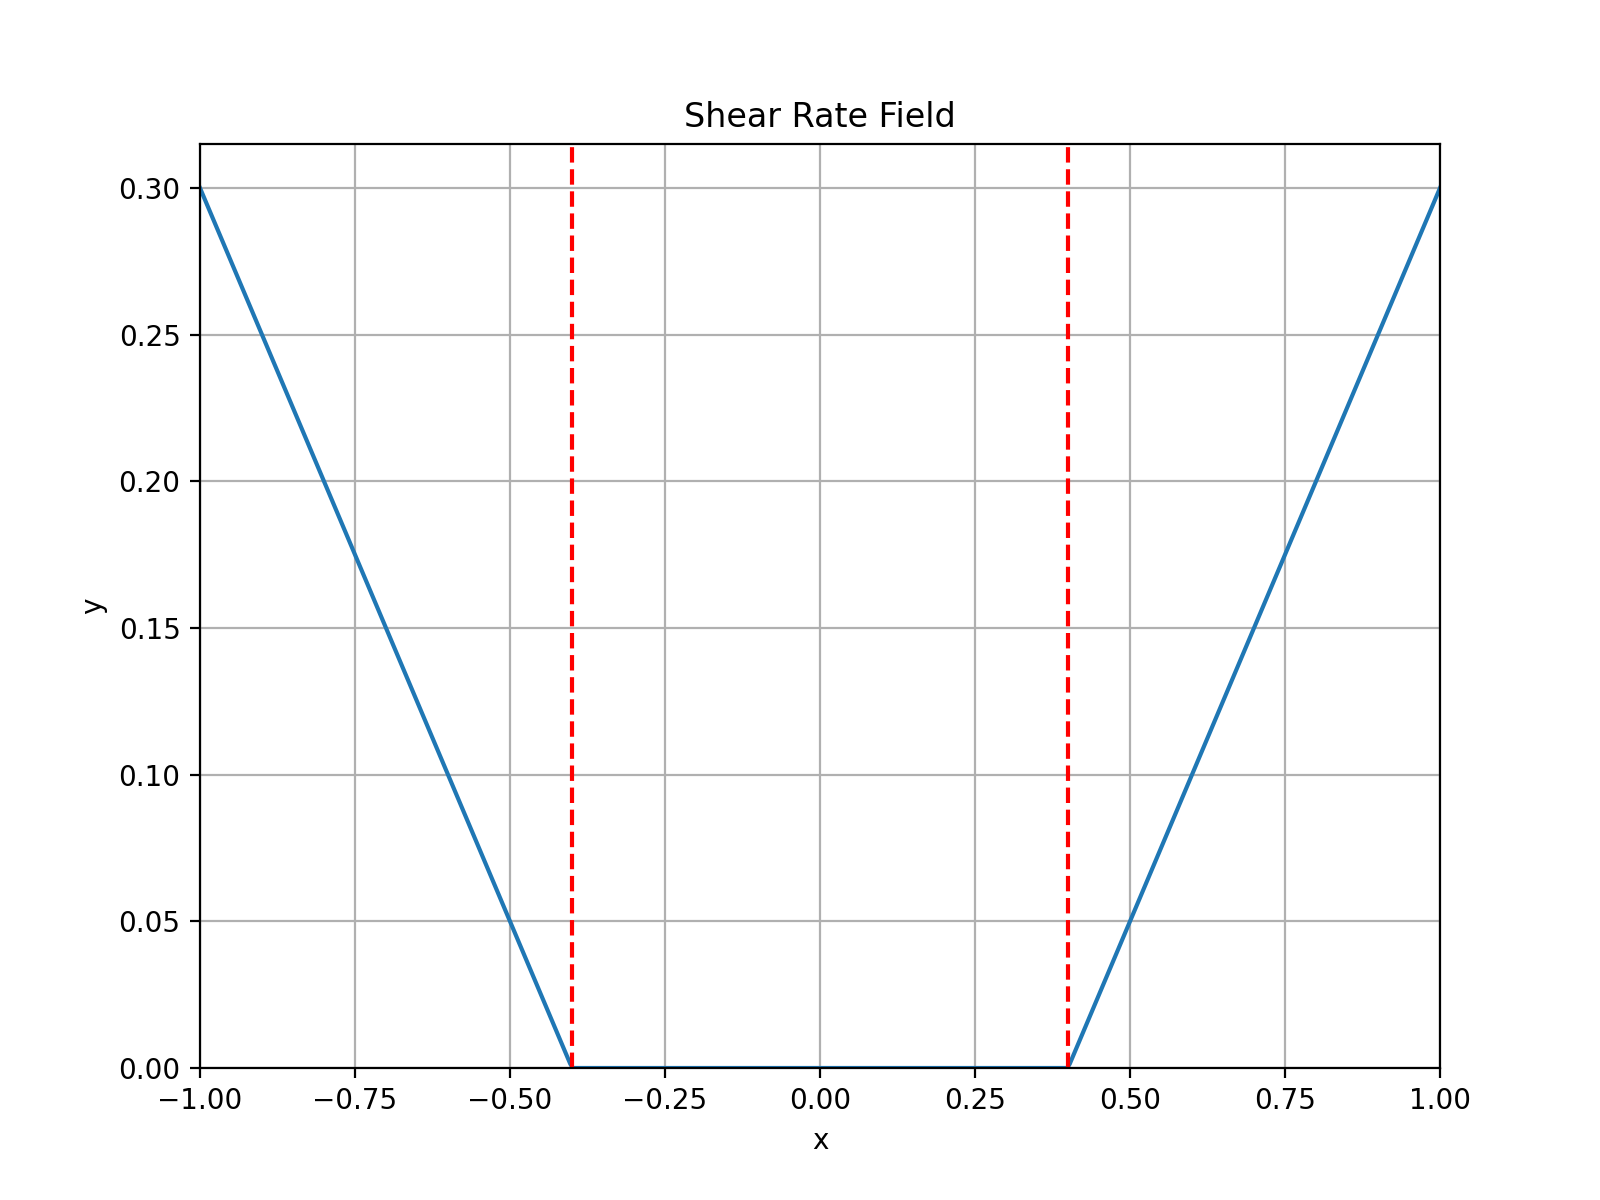
\includegraphics[width=0.8\textwidth]{figures/shear_rate_field.png}
%	\caption{Shear rate field for a Bingham fluid flowing through a tube.}
%\end{figure}
%\begin{figure}[ht]
%	\centering
%	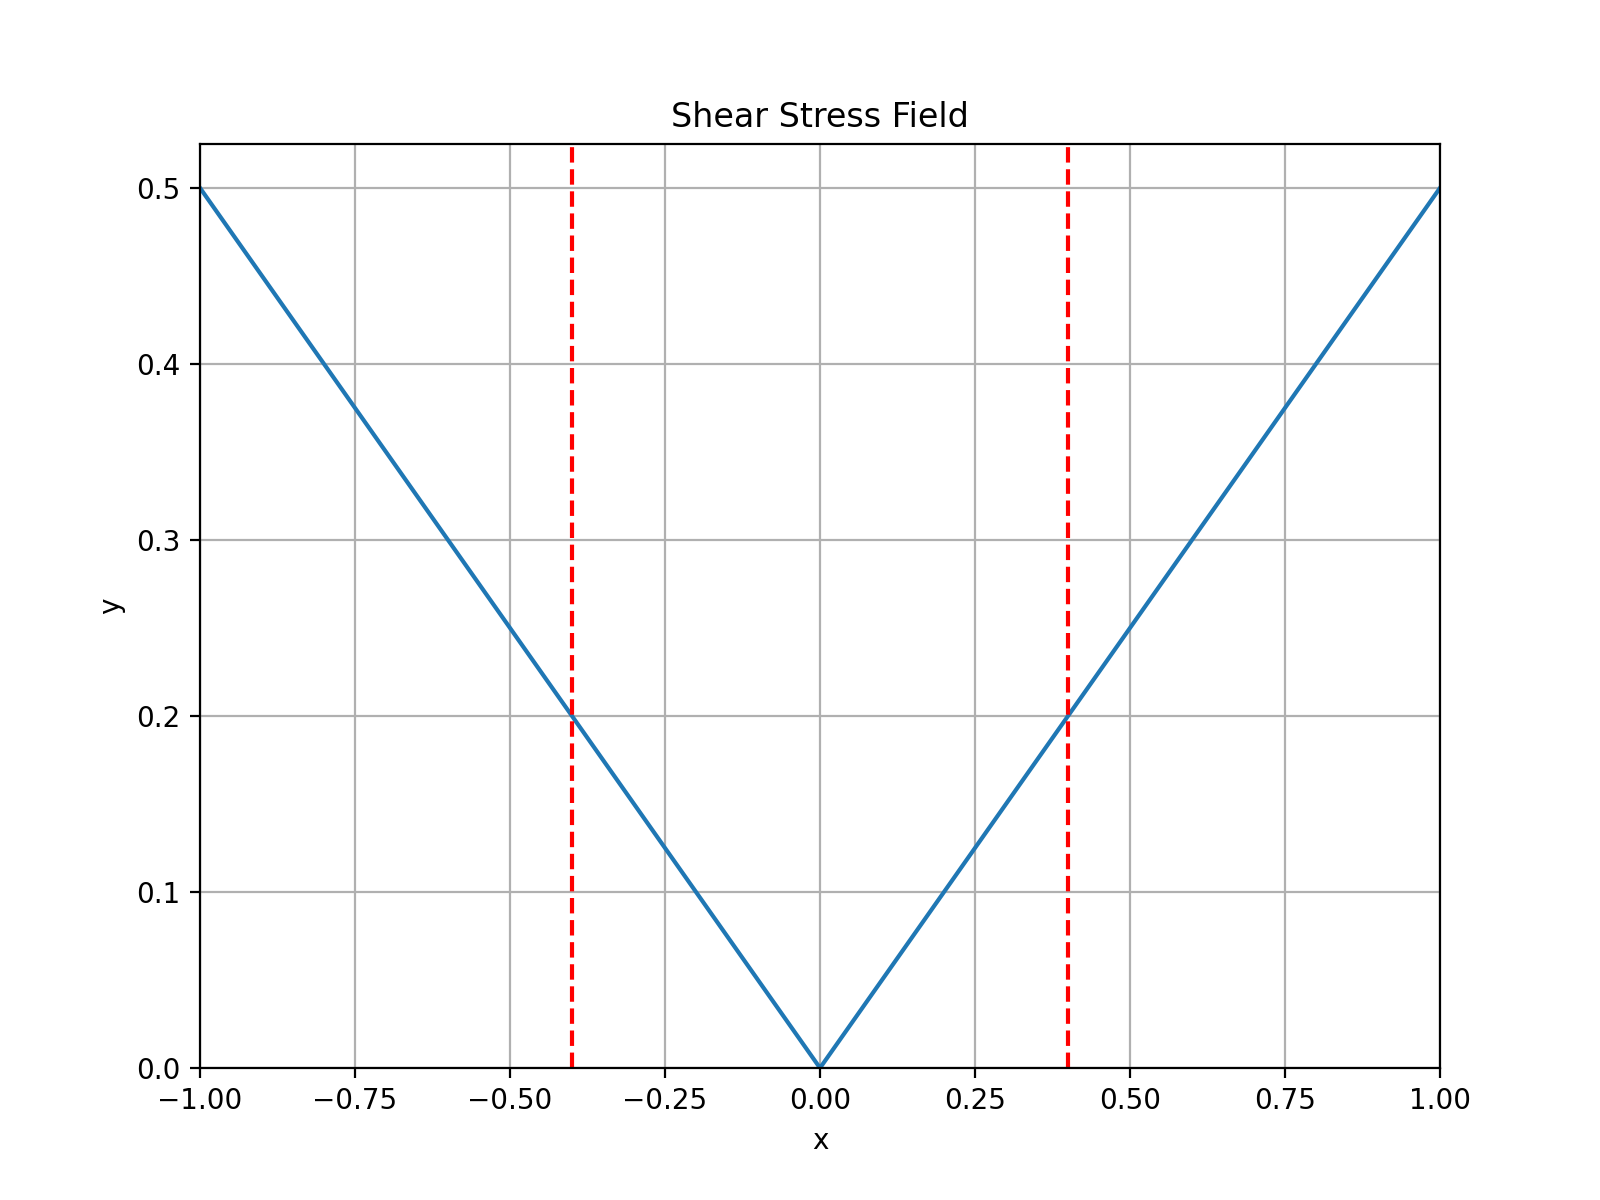
\includegraphics[width=0.8\textwidth]{figures/shear_stress_field.png}
%	\caption{Shear stress field for a Bingham fluid flowing through a tube.}
%\end{figure}
\begin{figure}[H]
	\centering
	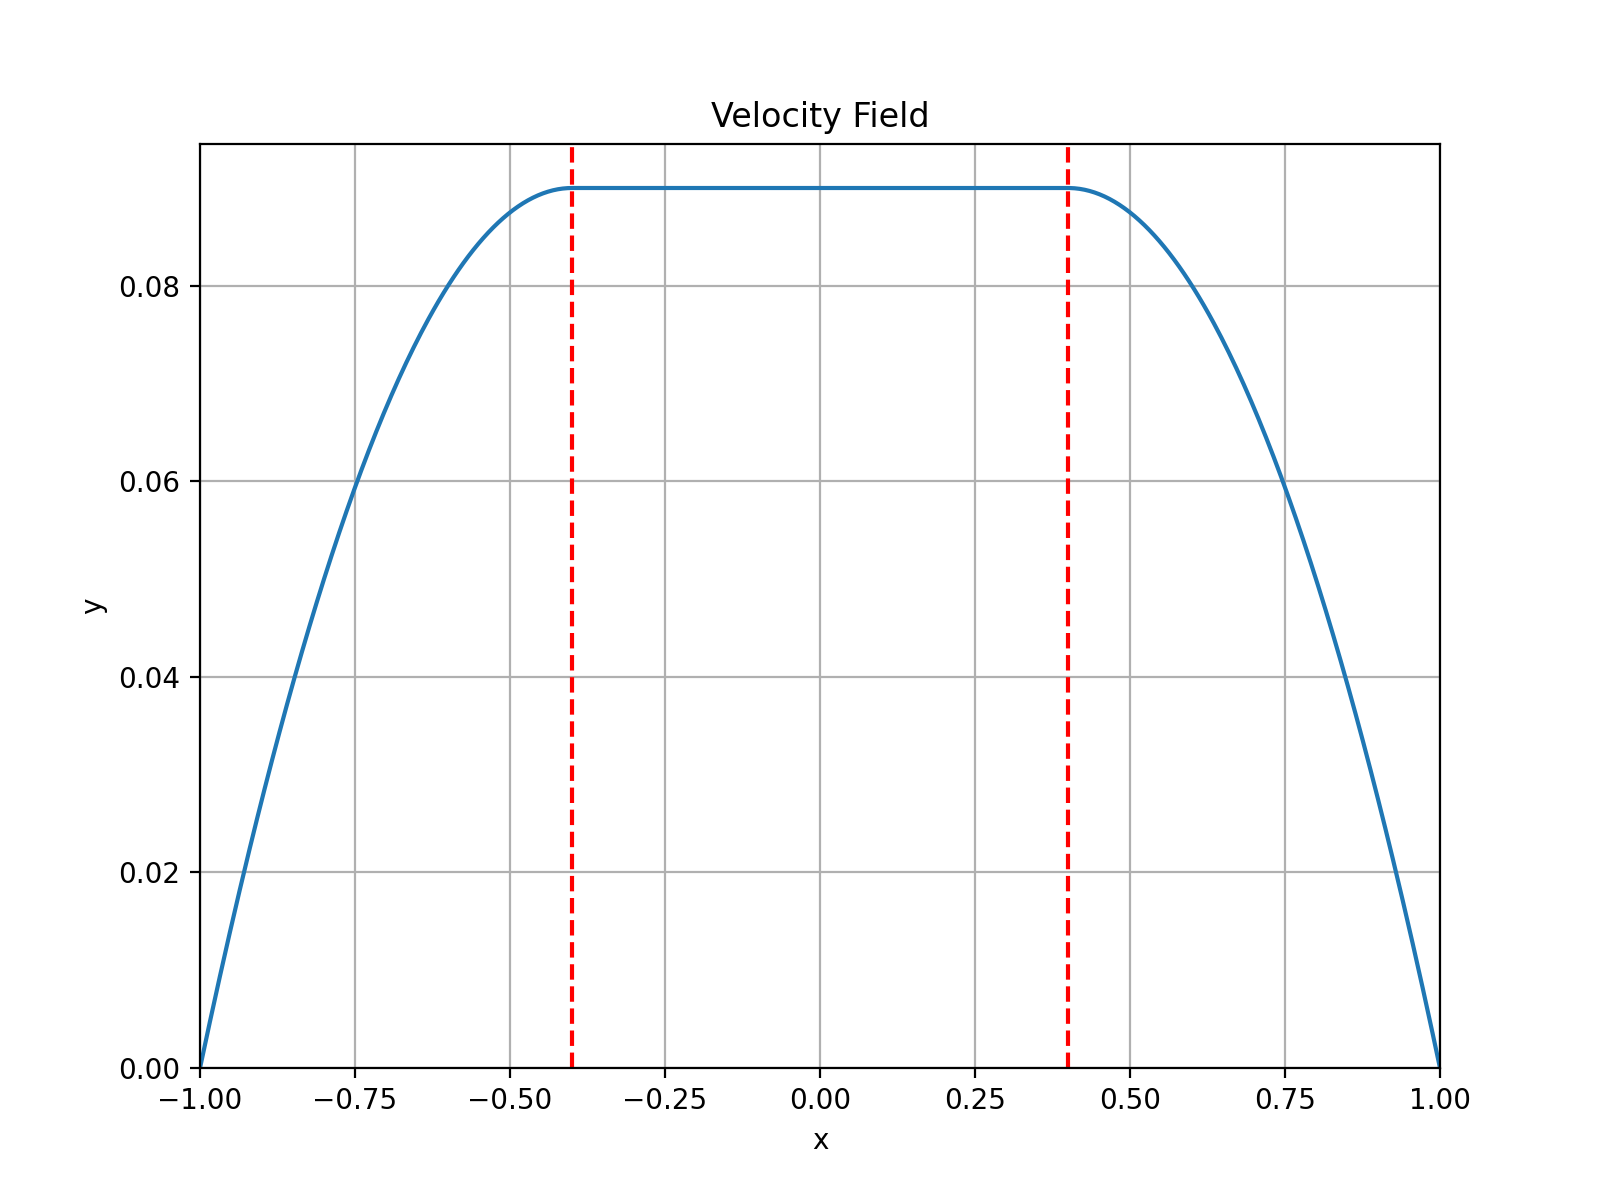
\includegraphics[width=0.8\textwidth]{figures/velocity_field.png}
	\caption{Velocity field for a Bingham fluid flowing through a tube.}
	\label{fig:malkin_3_9_velocity_field}
\end{figure}
\begin{figure}[H]
	\centering
	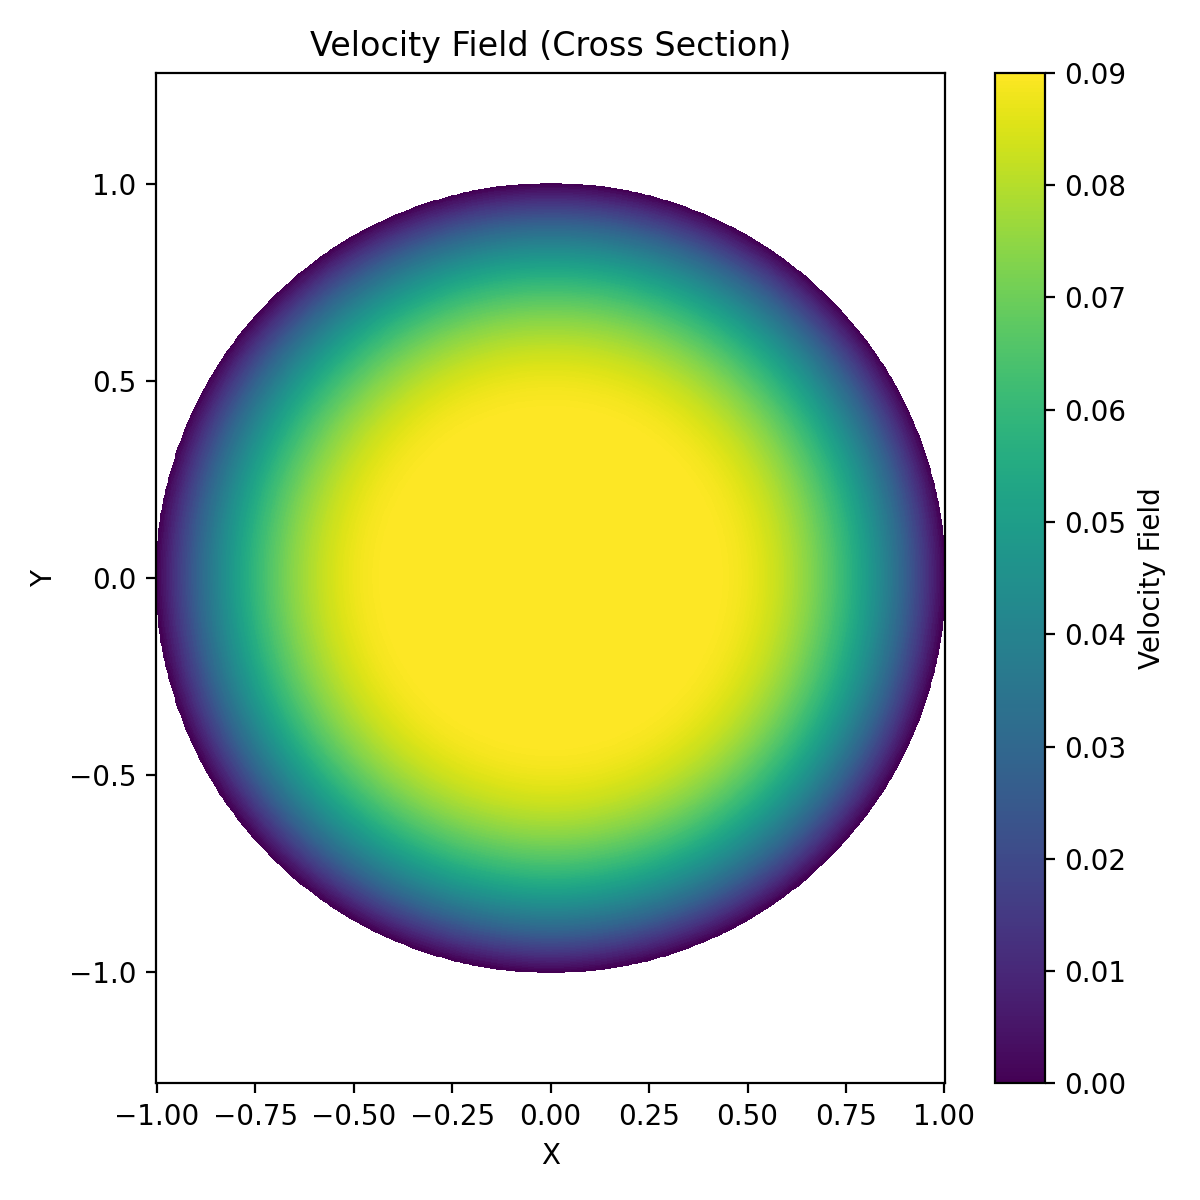
\includegraphics[width=0.32\textwidth]{figures/velocity_field_cross_section.png}
	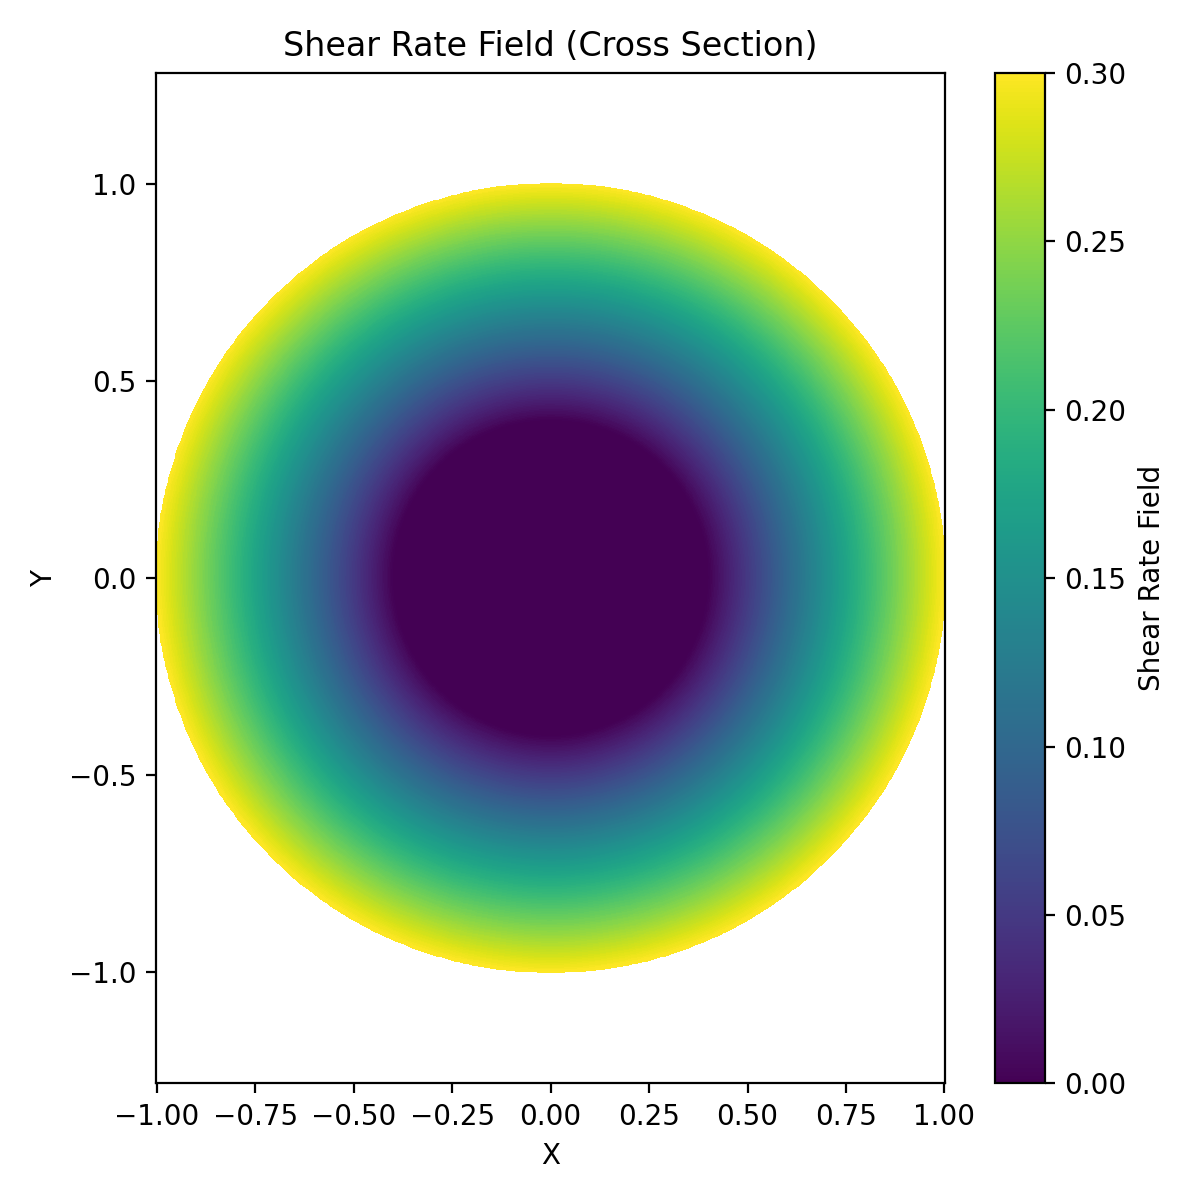
\includegraphics[width=0.32\textwidth]{figures/shear_rate_field_cross_section.png}
	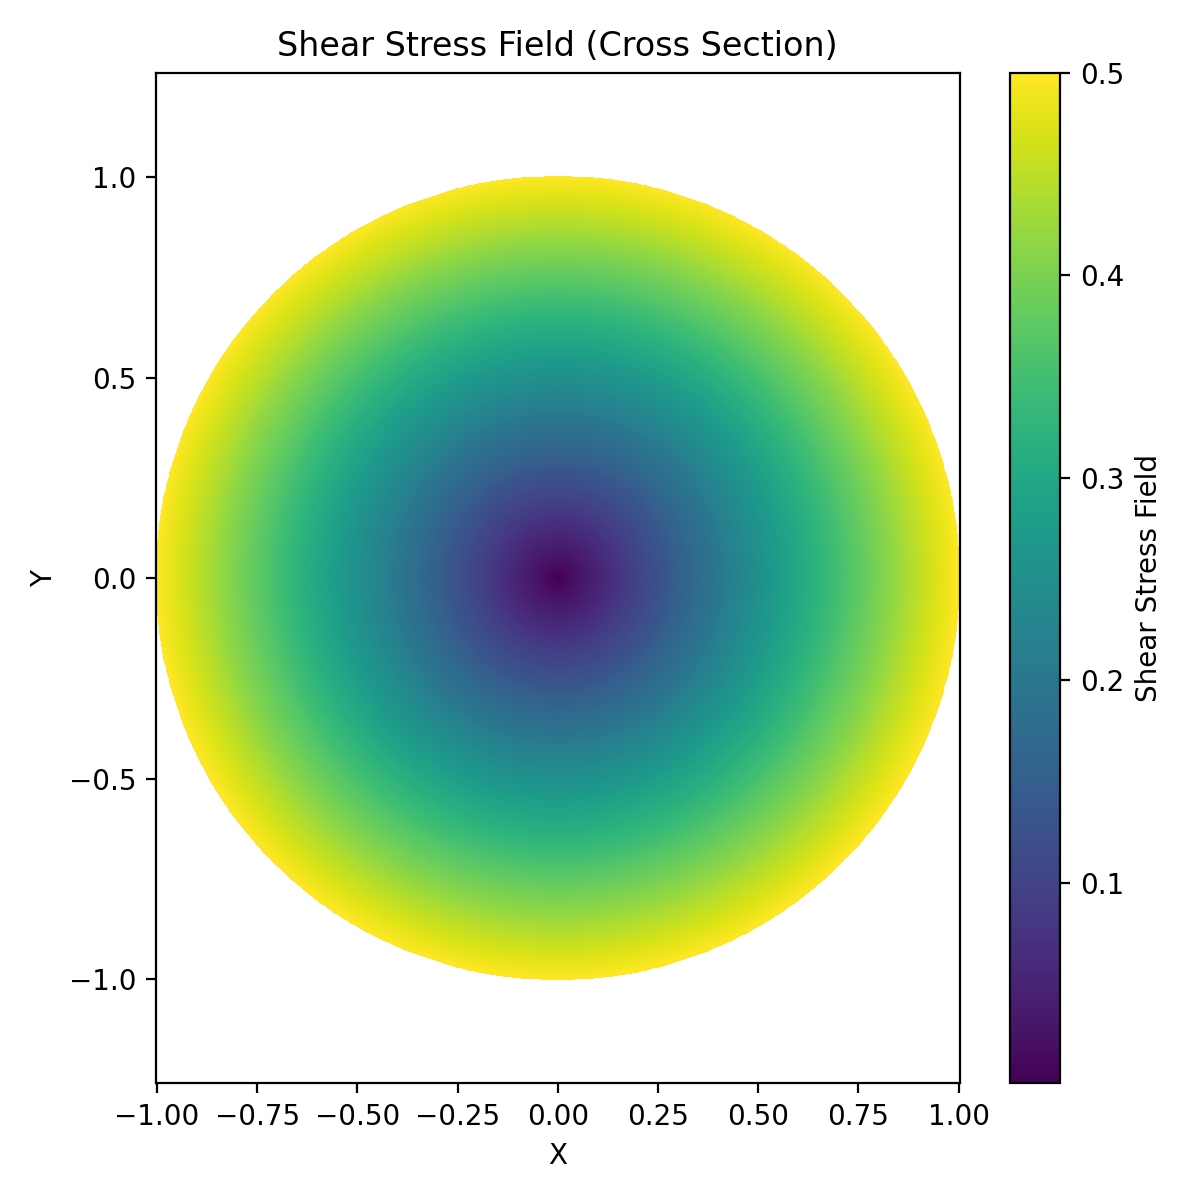
\includegraphics[width=0.32\textwidth]{figures/shear_stress_field_cross_section.png}
	\caption{Cross-sectional profiles of velocity, shear rate, and shear stress for a Bingham fluid flowing through a tube. The region near the center of the tube (where $r < r_0$) has zero shear rate. The velocity profile is flat in this region and then decreases towards the walls of the tube. The shear stress increases linearly with radius and exceeds the yield stress $\sigma_Y$ at $r = r_0$.}
	\label{fig:malkin_3_9_cross_section}
\end{figure} 




\section{5-7 Malkin}
\textit{In the principal scheme of measuring viscoelastic properties of the material, a spring is used (Fig. 5.7.1) that is not ideal elastic but viscoelastic (has some losses in deformation). How do you calculate the viscoelastic properties of the material under investigation?}

The solution for the driving oscillator $x_1$ and the top plate $x_2$ are:
\[
	\begin{bmatrix}
		x_1 \\ x_2
	\end{bmatrix}
	=
	\begin{bmatrix}
		c_1 \\ c_2 e^{i\varphi}
	\end{bmatrix}
	e^{i\omega t}
\]
For the top plate we have:
\[
	m\ddot{x}_2 + Z^* x_2 + \frac{S}{h}G^*(x_2 - x_1) = 0
\]
where $m$ is the mass of the top plate, $Z^*$ is the complex modulus of the spring, 
$G^*$ is the complex modulus of the material, $S$ is the surface area of the plate 
and $h$ is the height of the sample. Since the spring has a non-zero loss modulus, 
$Z^* = Z' + iZ''$ is complex.

Substituting $x_1 = c_1 e^{i\omega t}$, $x_2 = c_2 e^{i\varphi} e^{i\omega t}$ 
and $\ddot{x}_2 = -c_2\omega^2 e^{i\varphi} e^{i\omega t}$:
\[
	-mc_2\omega^2 e^{i\varphi} + c_2 Z^* e^{i\varphi} 
	+ \frac{S}{h}G^*\left(c_2 e^{i\varphi} - c_1\right) = 0
\]
Solving for $G^*$:
\[
	\frac{S}{h}G^*\left(c_2 e^{i\varphi} - c_1\right) 
	= mc_2\omega^2 e^{i\varphi} - c_2 Z^* e^{i\varphi}
\]
\[
	G^* = \frac{h}{S} \cdot \frac{m\omega^2 - Z^*}{1 - \dfrac{c_1}{c_2}e^{-i\varphi}}
\]
For simplicity, let $r = c_1/c_2$. Separating real and imaginary components:
\[
	G^* = \frac{h}{S} \cdot 
	\frac{m\omega^2 - Z' - iZ''}{(1 - r\cos\varphi) + ir\sin\varphi}
\]
\[
	G^* = \frac{h}{S} \cdot 
	\frac{
		\left[(m\omega^2 - Z')(1 - r\cos\varphi) - Z'' r\sin\varphi\right]
		+ i\left[Z''(1 - r\cos\varphi) + (m\omega^2 - Z')r\sin\varphi\right]
	}{
		(1 - r\cos\varphi)^2 + r^2\sin^2\varphi
	}
\]
Therefore:
\[
	G' = \frac{h}{S} \cdot 
	\frac{(m\omega^2 - Z')(1 - r\cos\varphi) - Z'' r\sin\varphi}
	{(1 - r\cos\varphi)^2 + r^2\sin^2\varphi}
\]
\[
	G'' = \frac{h}{S} \cdot 
	\frac{Z''(1 - r\cos\varphi) + (m\omega^2 - Z')r\sin\varphi}
	{(1 - r\cos\varphi)^2 + r^2\sin^2\varphi}
\]
The loss tangent is:
\[
	\tan\delta = \frac{G''}{G'} = 
	\frac{Z''(1 - r\cos\varphi) + (m\omega^2 - Z')r\sin\varphi}
	{(m\omega^2 - Z')(1 - r\cos\varphi) - Z'' r\sin\varphi}
\]




\end{document}
